View demo code of this section: \democode{05}{5.4.5}

\subsubsection{Background}

An overall reinforcement learning algorithm(RL) is composed of Agent, Environment, State, Action, and Reward. After the Agent executes an action, the Environment switches to a new State according to the Action and gives a Reward according to certain rules. After that, the Agent updates its decision-making process according to the obtained new State and Reward and gives a new Action, and so on, until the entire control process is completed. We denote $\pi_{\theta}$ as the policy function, $s$ as each state of the environment, $r$ as the reward in each state, and $a$ as the action of the agent. The architecture of RL is demonstrated in Fig.~\ref{RL_frame}.
\begin{figure}[ht]
  \centering
  \includegraphics[scale=0.4]{5.4.5_RL/RL.png}
  \caption{\label{RL_frame} The demonstration of RL working process.}
\end{figure}

We assumed an environment has $N$ different states. And we act action $a_{i-1}$ on state $s_{i-1}$ with the result $s_{i}$. The transition probability function from state $s_{i-1}$ to state $s_{i}$ can be $P(s_{i+1}|s_{i},a_{i})$. Meanwhile, there is a reward $r_i$ in each state calculated by reward function $R_i=R(a_i,s_i,s_{i-1})$. In the progress of environmental change, the reward expectation is only determined by the latest $state$, which is called the Markov decision process. Therefore, each $T$ step trajectory will be chosen by the agent with probability:

\begin{equation}
    \begin{split}
        &P(\tau|\pi_{\theta})=\\
        &\rho(s_0)\prod_{k=0}^{k=T-1}P(s_{k+1}|s_{k},a_{k})\pi_{\theta}(a_{k}|s_{k}),
    \end{split}
\end{equation}
where $\rho$ is the initial state distribution. Then the expectation of $T$ steps trajectory's reward is:
\begin{equation}
    \eta(\pi_{\theta})=\int_{\tau}P(\tau|\pi_{\theta})R(\tau)d\tau.
\end{equation}
In order to get the optimal policy function $\pi_{\theta}$, the agent is trained to maximize the expectation $\eta$, which is:
\begin{equation}
    \pi_{\theta}^{opt}=\mathrm{argmax}_{\theta}\eta(\pi_{\theta}).
\end{equation}
In following sections, we will demonstrate how to train the agent in quantum device.

\subsubsection{Hybrid Deep Q-Network}

Replace the neural network in the classical Deep Q-network's agent with the quantum variational circuit, we get the hybrid deep Q-network(HDQN)~\cite{Q_rl}. The architecture of HDQN is illustrated in FIG.~\ref{HDQN}.

\begin{figure*}[ht]
    \centering
    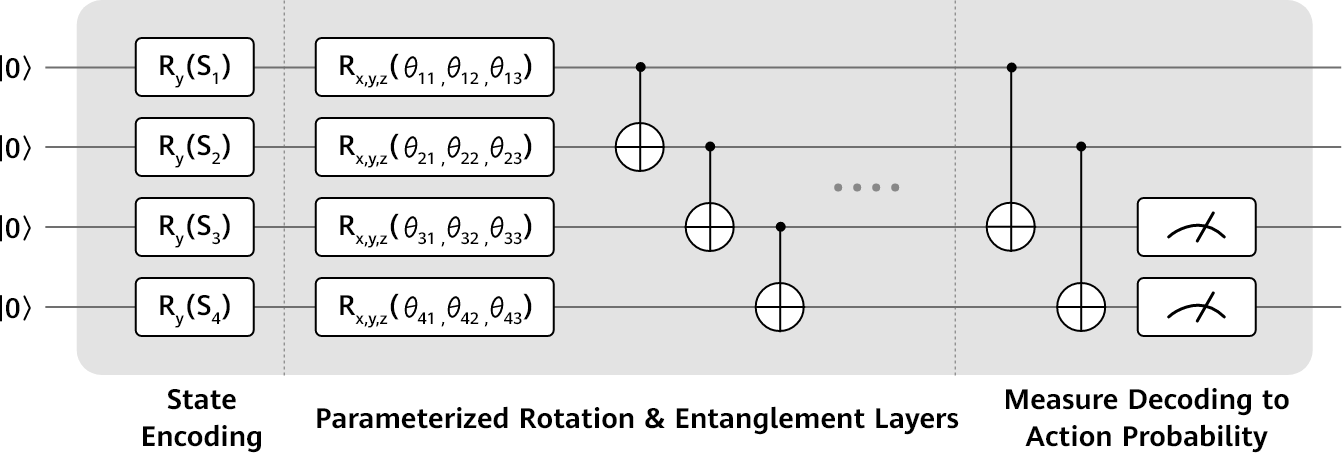
\includegraphics[scale=0.5]{5.4.5_RL/HDQN.png}
    \caption{\label{HDQN} The architecture of HDQN.}
  \end{figure*}

We calculate the parameters $\theta$ by classical neural network and use them to construct the quantum variational circuit. Finally, the quantum part applies the action to the environment. Meanwhile, the environment responds with a reward $r_i$. We denote $e_i=(s_i,a_i,r_{i+1},s_{i+1})$ as an experience. In the training stage, we will use these experiences as training samples to adjust the parameters in both the classical part and quantum part according to loss function $L(\theta)$:
\begin{equation}
\begin{split}
    L(\theta_{j})=&E[R_{i+1}+\\
    &\gamma \max_{\alpha^{'}}Q(s_{i+1},a^{'},\theta_{j}^{-})-Q(s_{i},a_{i},\theta_{i})^2].
\end{split}
\label{loss func}
\end{equation}

\textit{Variational quantum circuit} -- The variational quantum circuit is a quantum circuit using adjustable parameters that can be changed by the external environment. Here, according to the architecture in~\cite{Q_rl}, we construct the quantum circuit with the combination of encoder and ansatz. Here, we apply the Hardware Efficient circuit as the ansatz. The overall quantum circuit is illustrated in Fig.~\ref{Agent_qc}.

\begin{figure*}[ht]
  \centering
  \includegraphics[scale=0.5]{5.4.5_RL/Circuit.png}
  \caption{\label{Agent_qc} The overall quantum circuit of agent in RL.}
\end{figure*}

\textit{The implement in MindQuantum} -- Here, we give the example of realizing HDQN by \MindQuantum. The first step is to construct the quantum variational circuit including the encoder and the ansatz.
\begin{lstlisting}
def __get_encoder(self):
    encoder = Circuit()
    encoder += UN(H, 4)
    for i in range(4):
        encoder += RY(f'alpha{i}').on(i)
    encoder = encoder.no_grad()
    quantum circuit which has no gradient: no_grad()
    encoder.summary()
    return encoder
def __get_ansatz(self):
    ansatz = HardwareEfficientAnsatz\\
        (4, single_rot_gate_seq=[RX,RY,RZ],\\
        entangle_gate=X, depth=3).circuit
    ansatz += X.on(2,0)
    ansatz += X.on(3,1)
    ansatz.summary()
    return ansatz
self.circuit = self.encoder + self.ansatz
\end{lstlisting}

After the progress of the quantum circuit, we need to construct an observable Hamiltonian as a measurement basis. Here, we only measure the second and third qubits on $\sigma_y$ base. The Hamiltonian is as follows:
\begin{equation}
    H=I\otimes I\otimes\sigma_y\otimes\sigma_y.
\end{equation}
We can construct the Hamiltonian by \MindQuantum\ as follows:
\begin{lstlisting}
def __get_observable(self):
    hams=[Hamiltonian(QubitOperator(f'Y{i}'))\\
        for i in [2, 3]]
    return hams
\end{lstlisting}
Moreover, we can easily get the expectation and calculate the gradient of expectation by function \getexpectationwithgrad, which can be used to optimize parameters.

Next, we need to realize the classical part, which is a three-layers fully connected neural network with activation function rule.
\begin{lstlisting}
class Critic(nn.Cell):
    def __init__(self):
        super(Critic, self).__init__()
        self.relu = nn.ReLU()
        self.fc1 = nn.Dense(4, 64)
        self.fc2 = nn.Dense(64, 256)
        self.fc3 = nn.Dense(256, 1)

    def construct(self, x):
        x = self.relu(self.fc1(x))
        x = self.relu(self.fc2(x))
        x = self.fc3(x)
        return x
\end{lstlisting}

\textit{Environment} -- Here, we focus on the problem of the gym game "CartPole-v0". It's a game that has an unbalanced cart on a track. This game has two inputs $0$ and $1$, which correspond to two directions left and right respectively. Users should control the trace moving toward these two directions and keep the cart balanced as long as possible.

The first step is to create the environment by gym.
\begin{lstlisting}
import gym
env = gym.make('CartPole-v0')
\end{lstlisting}
\textit{Memory buffer} -- In the progress of training, the training samples are randomly selected from the previous experience $e_i$. Therefore, we need to construct a buffer to store and sample the experience $e_i$.
\begin{lstlisting}
class Memory(object):
    ......
\end{lstlisting}

\subsubsection{Training}
The final step is model training. At first, we initialize HDQN with random parameters and let the actor interact with the environment. Next, we store the interaction result in the memory buffer as training samples. Finally, we sample from the memory buffer and adjust the parameters both in the classical part and quantum part with loss function (\ref{loss func}). Because of the space limitation, we will not provide the detailed code here.

\textit{Result of numerical simulation} -- In order to evaluate the result of the HDQN. We do some experiments to evaluate the performance. As shown in Fig.~\ref{stochastic} We compare the average results from multiple experiments with randomized strategy experiments. The results show that reinforcement learning using quantum circuits as the agent has indeed learned the strategy.
\begin{figure}[ht]
  \centering
  \includegraphics[scale=0.3]{5.4.5_RL/result_paper.jpg}
  \caption{\label{stochastic} Comparison between RL and randomized strategy.}
\end{figure}
